\documentclass{article}
\title{\LaTeX Math notes}
\author{Samuel Hautamäki}
\date{th of April 2025}
\usepackage{mathtools,amssymb,amsthm,gensymb,textcomp}
\usepackage{graphicx}
\graphicspath{ {./images/} }
\begin{document}
  \maketitle
   
  \section{Bayes' theorem} 
  HL p 689\\
  condition is marked by $|$\\
  $P(A|B)=\frac{P(A\cap B)}{P(B)}$ use tree diagram.\\
  Example may 2012,5,hl p1\\
  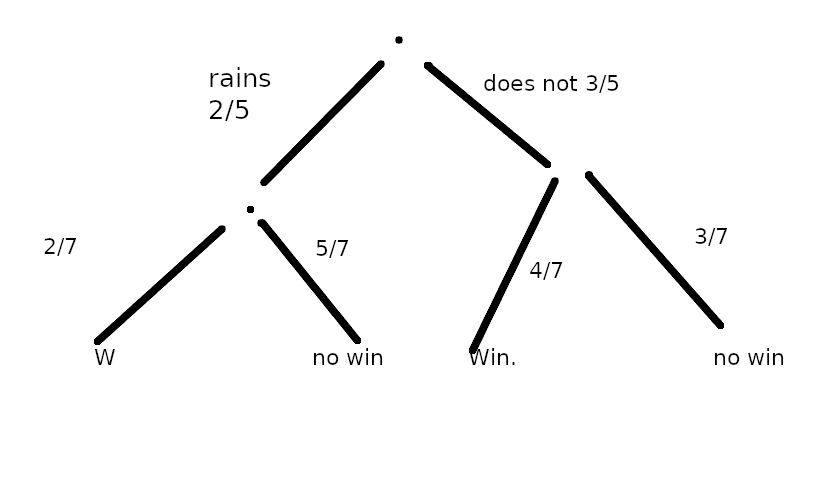
\includegraphics {tigers-rain}
  b) P(tigers win on a rainy day OR non-rainy day)=$\frac{2}{5}\cdot (\frac{2}{7})+\frac{3}{5}\cdot\frac{4}{7}$\\
  $\frac{4+12}{35}=\frac{16}{35}$\\
  c) Given that means the condition!\\
  $P(rainy day | Tigers won)=\frac{P(rainy day \cap Tigers won)}{P(tigers won)}=\frac{\frac{2}{5}\cdot\frac{2}{7}}{\frac{16}{35}}=\frac{\frac{4}{35}}{\frac{16}{36}}=\frac{4}{35}\cdot(\frac{35}{16})=\frac{4}{16}=\frac{1}{4}$\\
  HL 11C, p 695\\
  ex 1.\\
  P(yellow)=$P(both yellow)P(yellow | both yellow)+P(one of each)P(yellow | one of each)+P(both green)P(yellow | both green)$\\
  $=\frac{\frac{5}{2}}{\frac{13}{2}}\cdot \frac{4}{10}\frac{\frac{5}{1}+\frac{8}{1}}{\frac{13}{2}}\cdot\frac{3}{10}+\frac{\frac{8}{2}}{\frac{13}{2}}\cdot\frac{2}{10}=\frac{18}{65}$\\
  $P(yellow from A|yellow)=\frac{\frac{5}{2}}{\frac{13}{2}}\cdot\frac{2}{4}+\frac{\frac{5}{1}\frac{8}{1}}{\frac{13}{2}}\cdot\frac{1}{3}+\frac{\frac{8}{2}}{\frac{13}{2}}\cdot0=\frac{55}{234}$\\
  

   
\end{document}
